\documentclass{article}

\usepackage[paperwidth=90cm,paperheight=150cm,margin=2.0cm]{geometry}
\usepackage{graphicx}
\usepackage{xcolor}
\usepackage{tikz}
\usepackage{eso-pic}
\usepackage{tcolorbox}
\tcbuselibrary{skins}
\usepackage{booktabs}
\usepackage{array}
\usepackage{enumitem}
\usepackage{fontspec}
\usepackage{xfp}

\setmainfont{Times New Roman}
\setsansfont{Arial}

\pagestyle{empty}
\setlength{\parindent}{0pt}
\setlength{\parskip}{0.25em}
\setlist[itemize]{leftmargin=1.2em,itemsep=0.15em,topsep=0.15em}
\setlist[enumerate]{leftmargin=1.2em,itemsep=0.15em,topsep=0.15em}

\definecolor{theme}{RGB}{160,78,9}
\definecolor{themeDark}{RGB}{120,55,5}
\definecolor{posterBgTop}{RGB}{255,255,255}
\definecolor{posterBgBottom}{RGB}{247,196,132}

% Change this single number to scale all poster fonts together.
% Example: 1.05 makes all text 5% larger; 0.95 makes all text 5% smaller.
\newcommand{\FontScale}{1.25}
\newcommand{\scaledfontsize}[2]{%
  \fontsize{\fpeval{#1*\FontScale}pt}{\fpeval{#2*\FontScale}pt}\selectfont
}

\newcommand{\bodyfont}{\scaledfontsize{35}{42}}
\newcommand{\smallbodyfont}{\scaledfontsize{31.5}{38}}
\newcommand{\captionfont}{\scaledfontsize{29.5}{35}}

\newtcolorbox{sectionbox}[1]{
  enhanced,
  colback=white,
  colframe=theme,
  boxrule=1.1mm,
  arc=3mm,
  left=6mm,
  right=6mm,
  top=5mm,
  bottom=5mm,
  title={#1},
  fonttitle=\bfseries\sffamily\scaledfontsize{42}{50},
  coltitle=white,
  colbacktitle=theme,
  attach boxed title to top left={xshift=0mm,yshift=0mm},
  boxed title style={
    sharp corners,
    boxrule=0mm,
    colback=theme,
    left=7mm,
    right=7mm,
    top=3.5mm,
    bottom=3.5mm
  }
}

\newtcolorbox{introbox}{
  enhanced,
  colback=theme,
  colframe=theme,
  boxrule=0mm,
  arc=3mm,
  left=7mm,
  right=7mm,
  top=6mm,
  bottom=6mm
}

\newcommand{\figcap}[1]{\\[-0.2em]{\captionfont #1}}

\begin{document}

\AddToShipoutPictureBG{%
  
\begin{tikzpicture}[remember picture,overlay]
    \path[
      shade,
      top color=posterBgTop,
      middle color=posterBgTop,
      bottom color=posterBgBottom
    ] (current page.north west) rectangle (current page.south east);
  \end{tikzpicture}%
}

\begin{center}
  {\sffamily\bfseries\scaledfontsize{63}{75} Data-Driven Modeling and Analysis of a Gas-Steam Combined Cycle}\\[0.45em]
  {\scaledfontsize{38}{46} Yichen Wang}\\[0.25em]
  {\itshape\scaledfontsize{33}{40} Xingjian College, Tsinghua University, Beijing 100084, China}\\[0.65em]
  \color{theme}\rule{0.96\linewidth}{1.2mm}
\end{center}

\vspace{0.45cm}

\begin{introbox}
{\color{white}\sffamily\bfseries\scaledfontsize{44}{53} Introduction}\\[0.45em]
{\color{white}\bodyfont
This study builds a thermodynamic analysis framework for a 2-on-1 gas-steam combined heat and power (CHP) unit based on field operation data (April--December 2025). The framework covers working-fluid modeling, gas-turbine and steam/water-side energy analysis, and whole-plant efficiency-factor analysis under both power-only and heating modes.}
\end{introbox}

\vspace{0.65cm}

\begin{minipage}[t][0.78\textheight][t]{0.488\linewidth}
\vspace{0pt}

\begin{sectionbox}{1. Working-Fluid Modeling}
\bodyfont
\begin{center}
  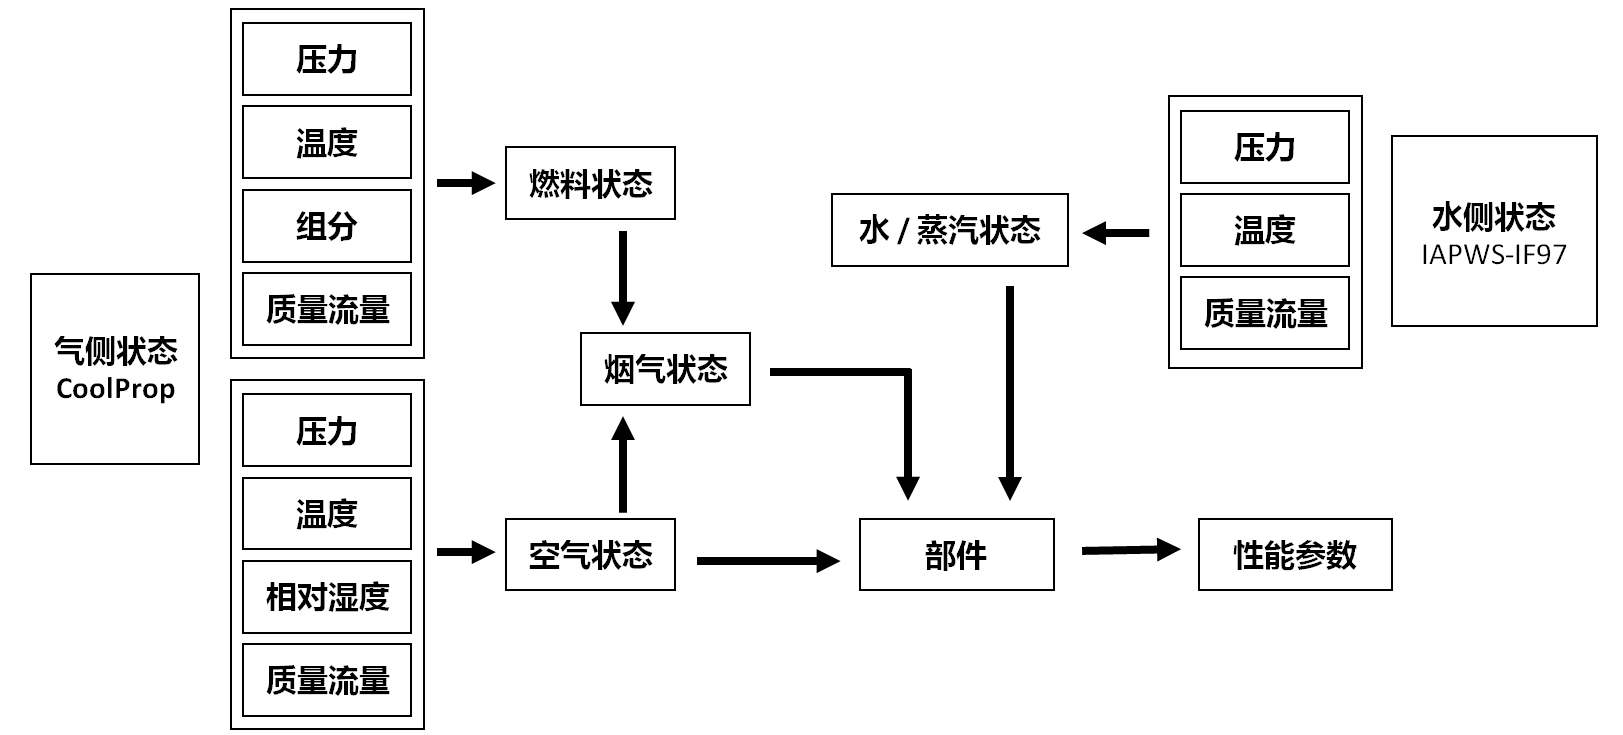
\includegraphics[width=0.75\linewidth]{../../thesis/figures0/chapter2/工质建模示意图.png}
  \figcap{Fig. 1. Working-fluid state and property modeling.}
\end{center}
\smallbodyfont
Gas, air, fuel, water, and steam streams are represented by unified flow-state objects. Thermodynamic properties such as enthalpy, entropy, energy flow, and exergy flow are calculated consistently for downstream component models.
\end{sectionbox}

\vspace{0.65cm}

\begin{sectionbox}{2. Gas-Turbine Analysis}
\bodyfont
\begin{center}
  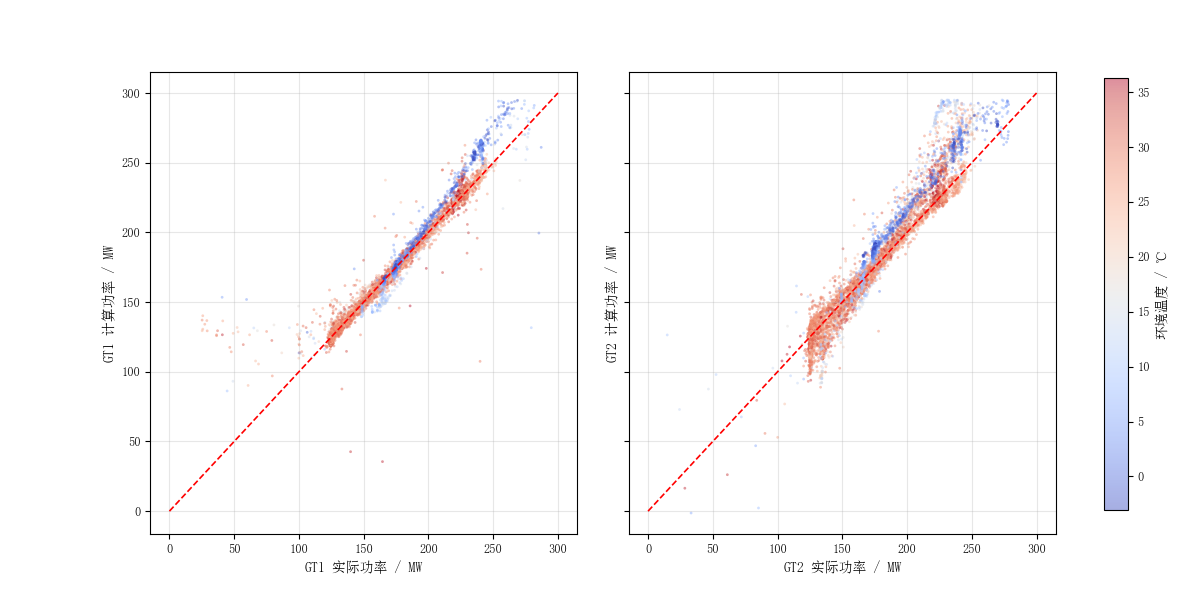
\includegraphics[width=0.84\linewidth]{../../thesis/figures0/chapter3/1燃机出力.png}
  \figcap{Fig. 2. Gas-turbine calculated and measured power.}
\end{center}
\vspace{0.25em}
\begin{center}
  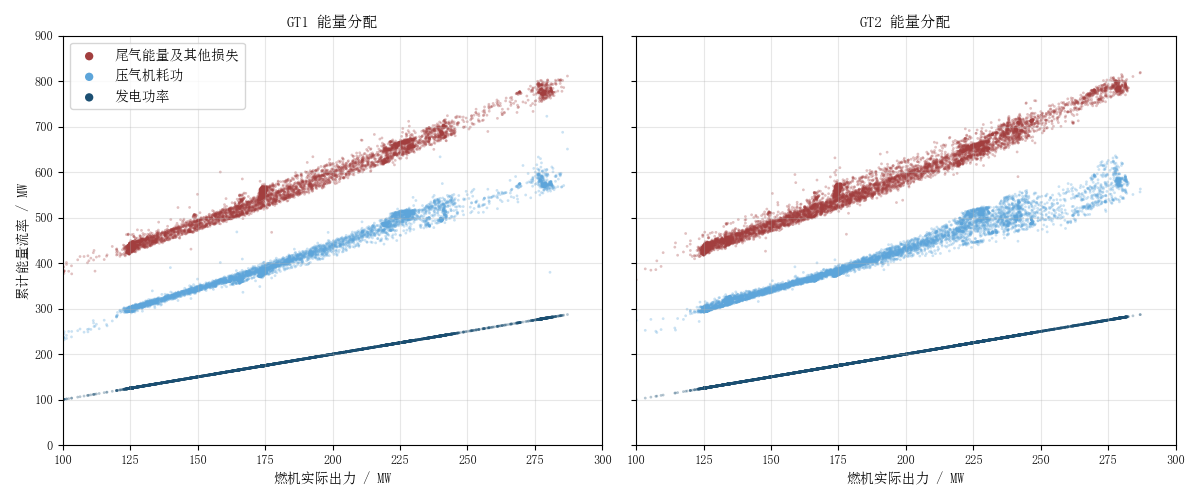
\includegraphics[width=0.84\linewidth]{../../thesis/figures0/chapter3/2能量分配散点图.png}
  \figcap{Fig. 3. Fuel-energy distribution in the gas turbine.}
\end{center}
\smallbodyfont
The gas-turbine model evaluates compressor work, turbine work, net power, fuel energy, and exhaust heat. The energy distribution clarifies how fuel input is divided into electric output, internal compression work, and recoverable exhaust energy.
\end{sectionbox}

\vspace{0.65cm}

\begin{sectionbox}{3. Steam/Water-Side Analysis}
\bodyfont
\begin{center}
  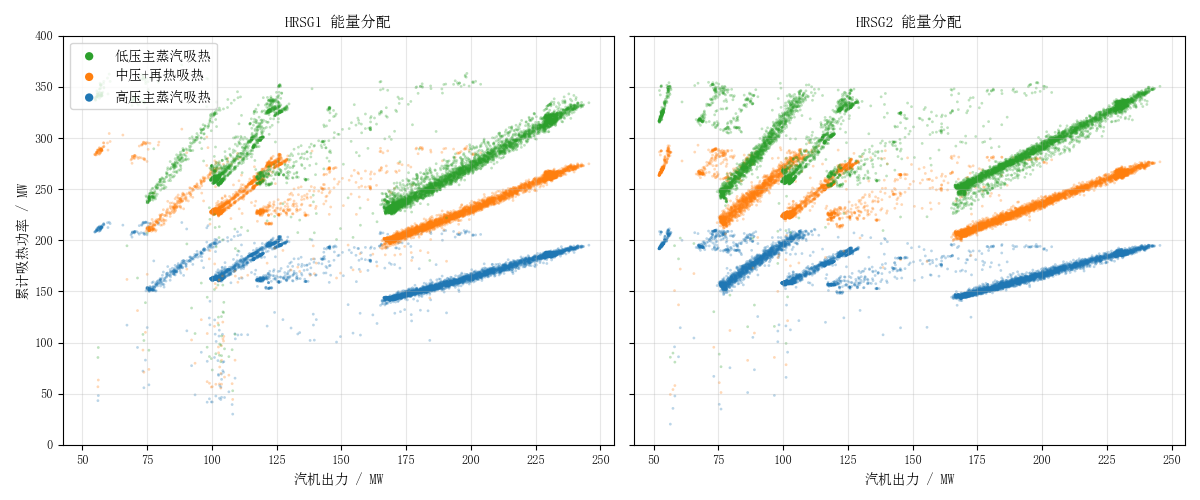
\includegraphics[width=0.84\linewidth]{../../thesis/figures0/chapter4/2水侧吸热分配.png}
  \figcap{Fig. 4. Heat absorption distribution on the steam/water side.}
\end{center}
\vspace{0.25em}
\begin{center}
  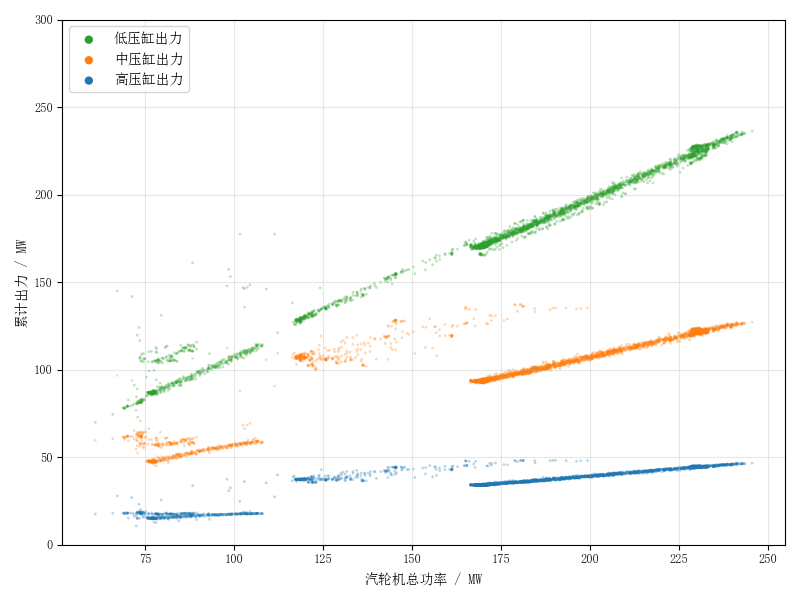
\includegraphics[width=0.65\linewidth]{../../thesis/figures0/chapter4/4各缸出力分配.png}
  \figcap{Fig. 5. Power distribution among HP, IP, and LP cylinders.}
\end{center}
\smallbodyfont
The HRSG transfers gas-side heat to high-pressure steam, intermediate-pressure/reheat steam, and low-pressure steam. The steam turbine further converts steam energy into cylinder power, while heating extraction changes the effective output definition.
\end{sectionbox}

\end{minipage}
\hspace{2.0cm}
\begin{minipage}[t][0.78\textheight][t]{0.488\linewidth}
\vspace{0pt}

\begin{sectionbox}{4. Whole-Plant Efficiency}
\bodyfont
\begin{center}
  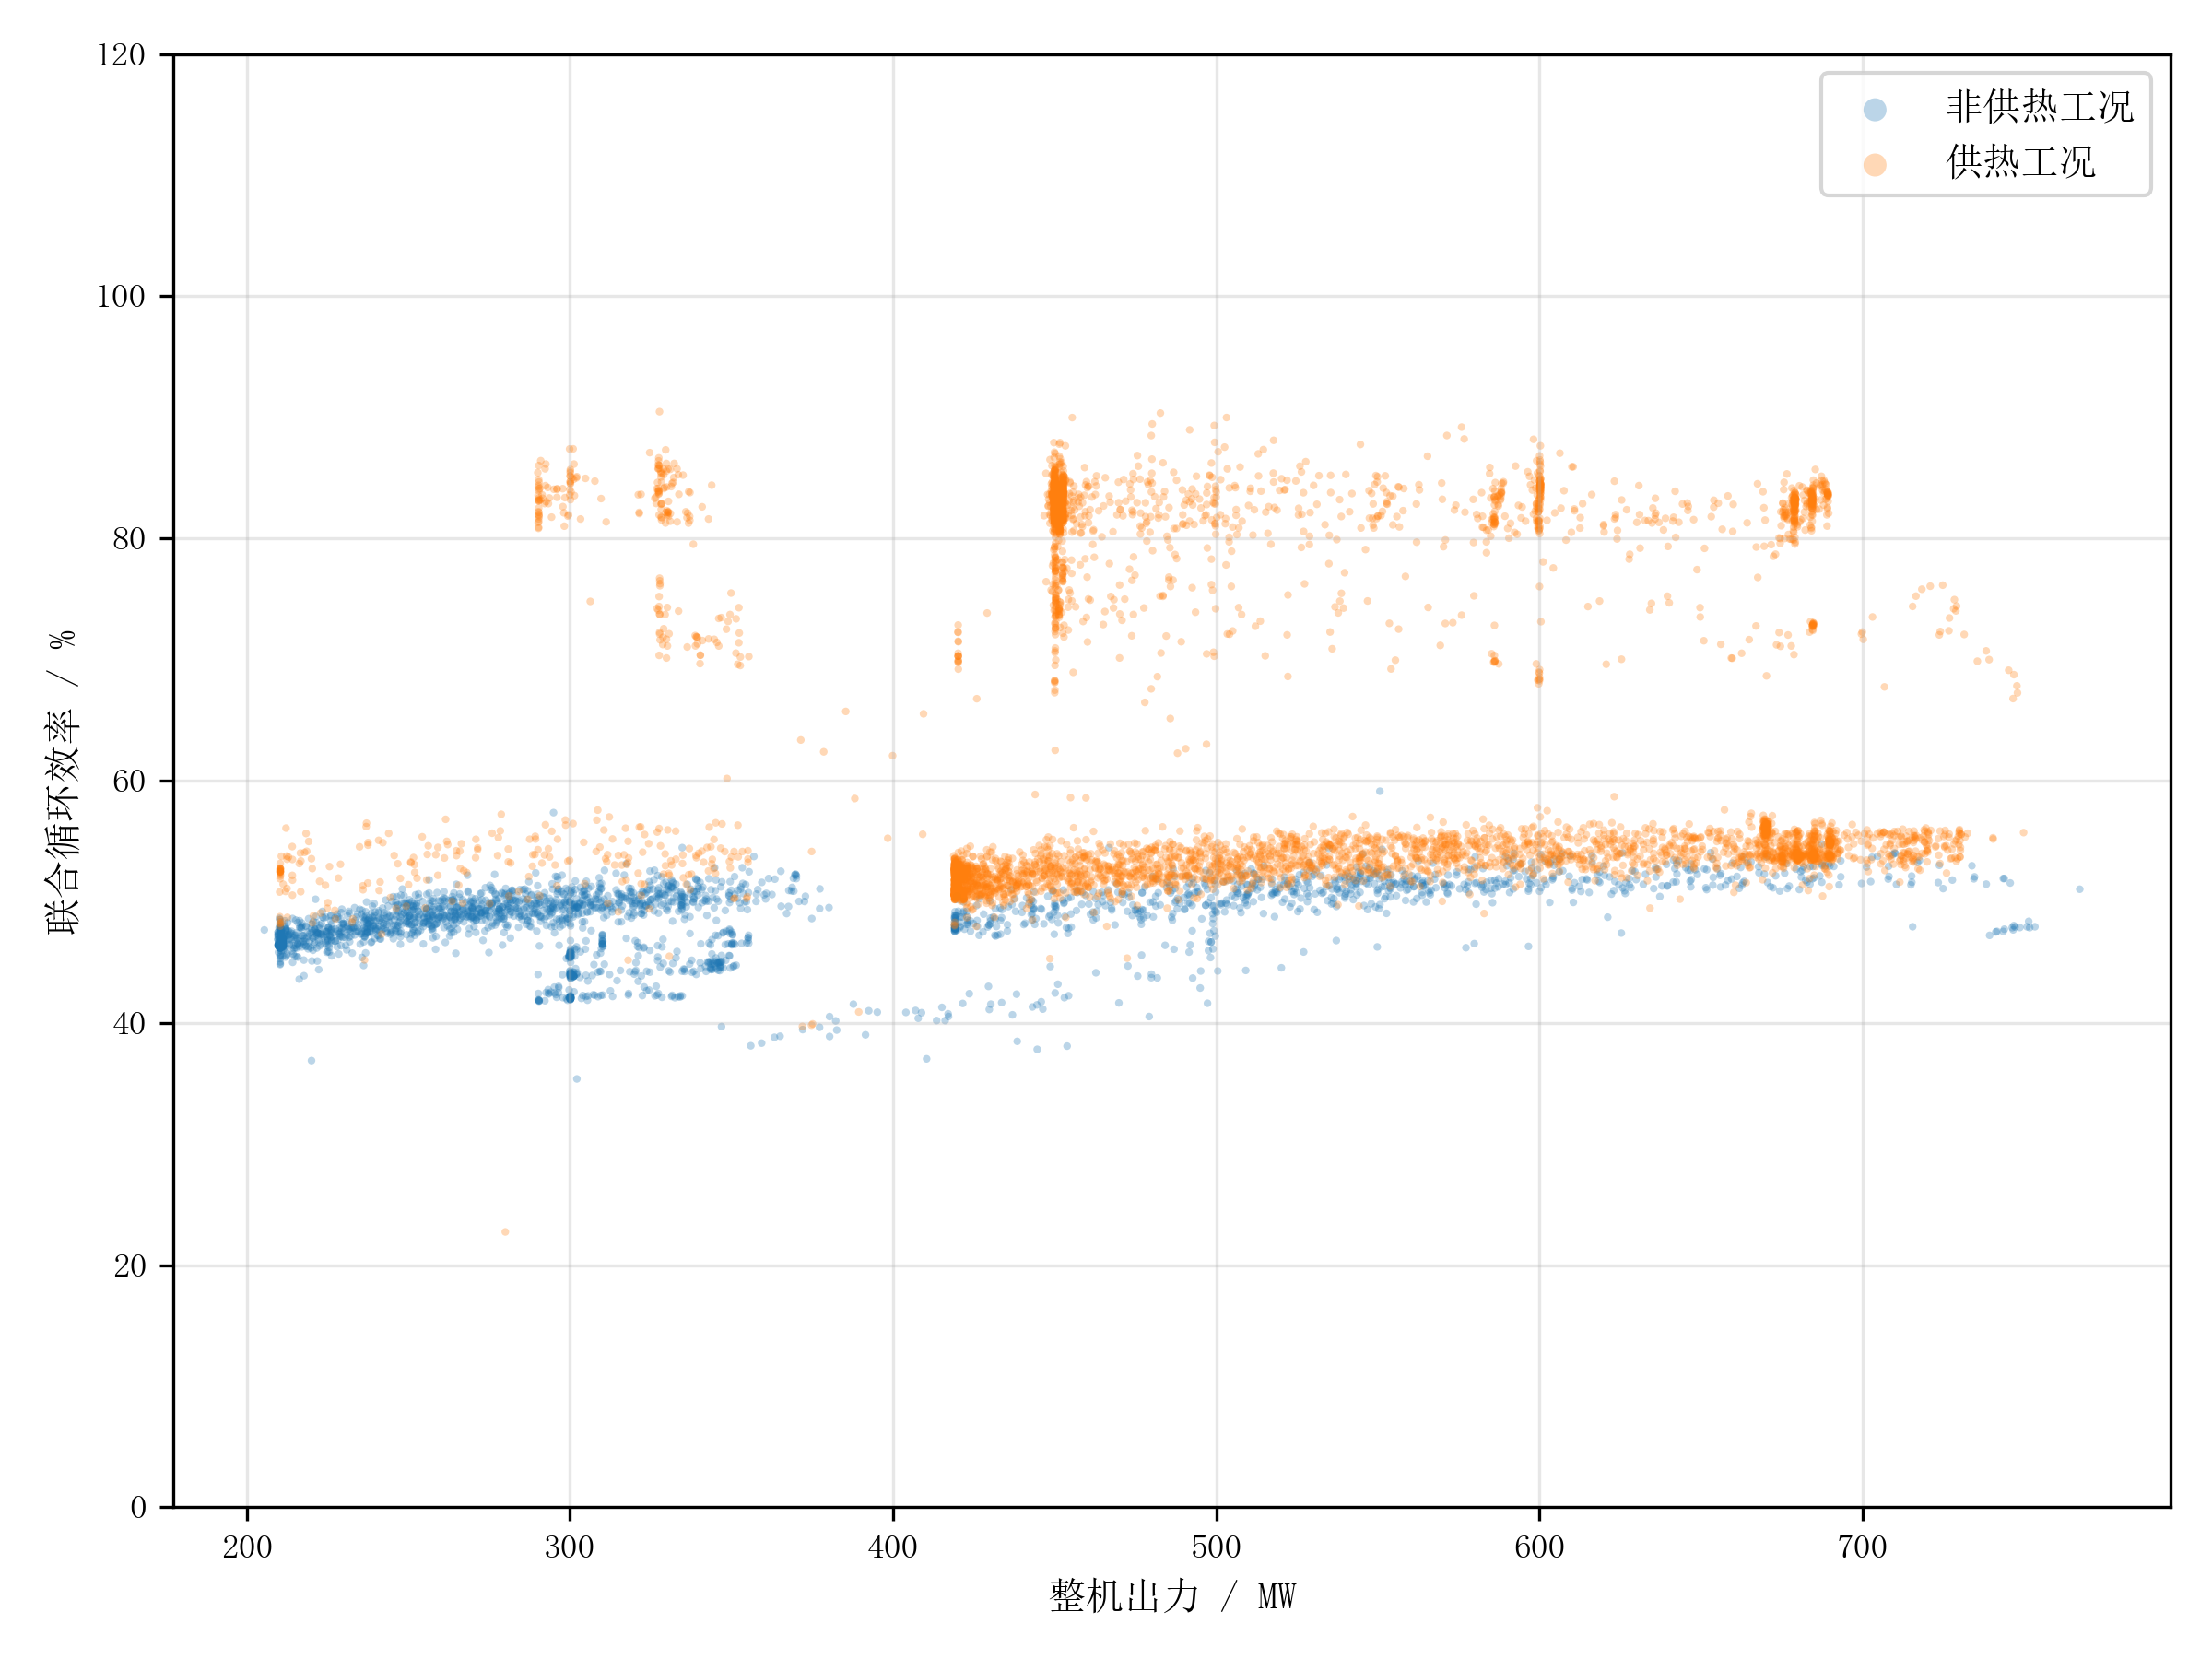
\includegraphics[width=0.8\linewidth]{../../thesis/figures0/chapter5/整机出力_效率关系.png}
  \figcap{Fig. 6. Combined-cycle efficiency versus total plant power.}
\end{center}
\smallbodyfont
Power-only samples cluster by single-GT versus dual-GT operation. Heating samples reach higher utilization because CHP efficiency counts heat supply as useful output: $\eta_{\mathrm{CHP}} = (W_{\mathrm{e}} + Q_{\mathrm{h}}) / Q_{\mathrm{f}}$.
\vspace{0.25em}
\begin{center}
  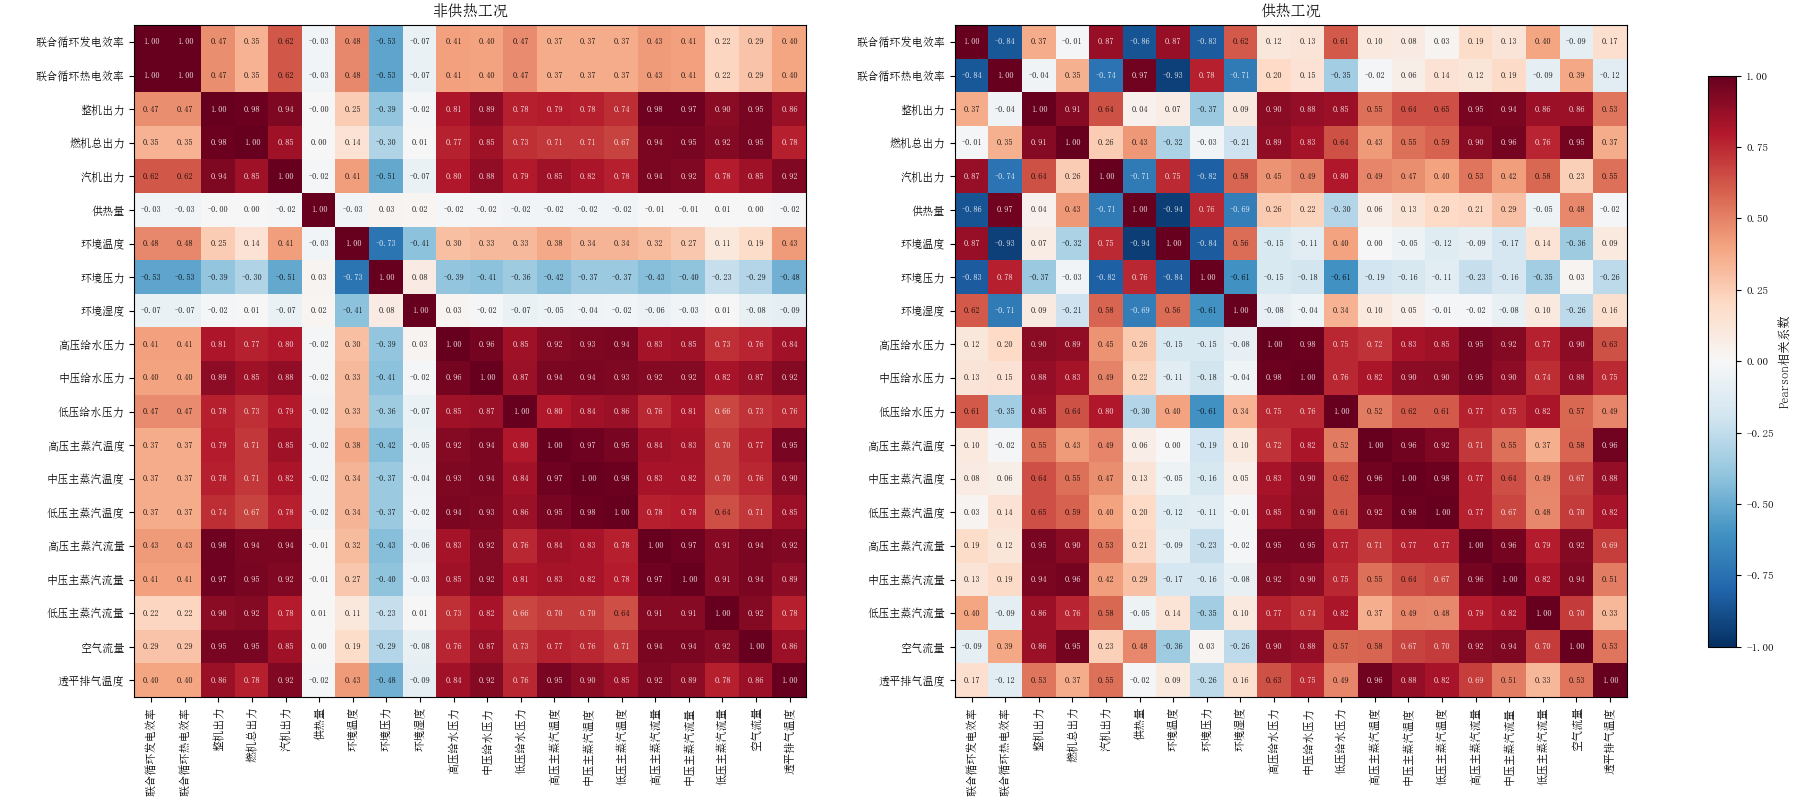
\includegraphics[width=0.86\linewidth]{../../thesis/figures0/chapter5/皮尔森系数矩阵.png}
  \figcap{Fig. 7. Pearson correlation matrices for power-only and heating modes.}
\end{center}
\smallbodyfont
The two modes are analyzed separately: power-only uses electric efficiency while heating uses CHP efficiency, since heat supply changes the numerator of the efficiency definition and reverses the sign of some correlations.
\end{sectionbox}

\vspace{0.65cm}

\begin{sectionbox}{5. Key Efficiency Factors}
\smallbodyfont
Pearson correlation and scatter-plot analyses identify the dominant factors for each mode. In power-only operation, efficiency correlates most with ST output, ambient pressure, and HP main-steam flow. In heating operation, CHP efficiency is dominated by heat supply ($r=0.966$) and ambient temperature ($r=-0.930$); ST output is negatively correlated ($r=-0.739$) because increased generation reduces heating extraction.
\vspace{0.2em}
\begin{center}
  \begin{minipage}[t]{0.48\linewidth}
    \centering
    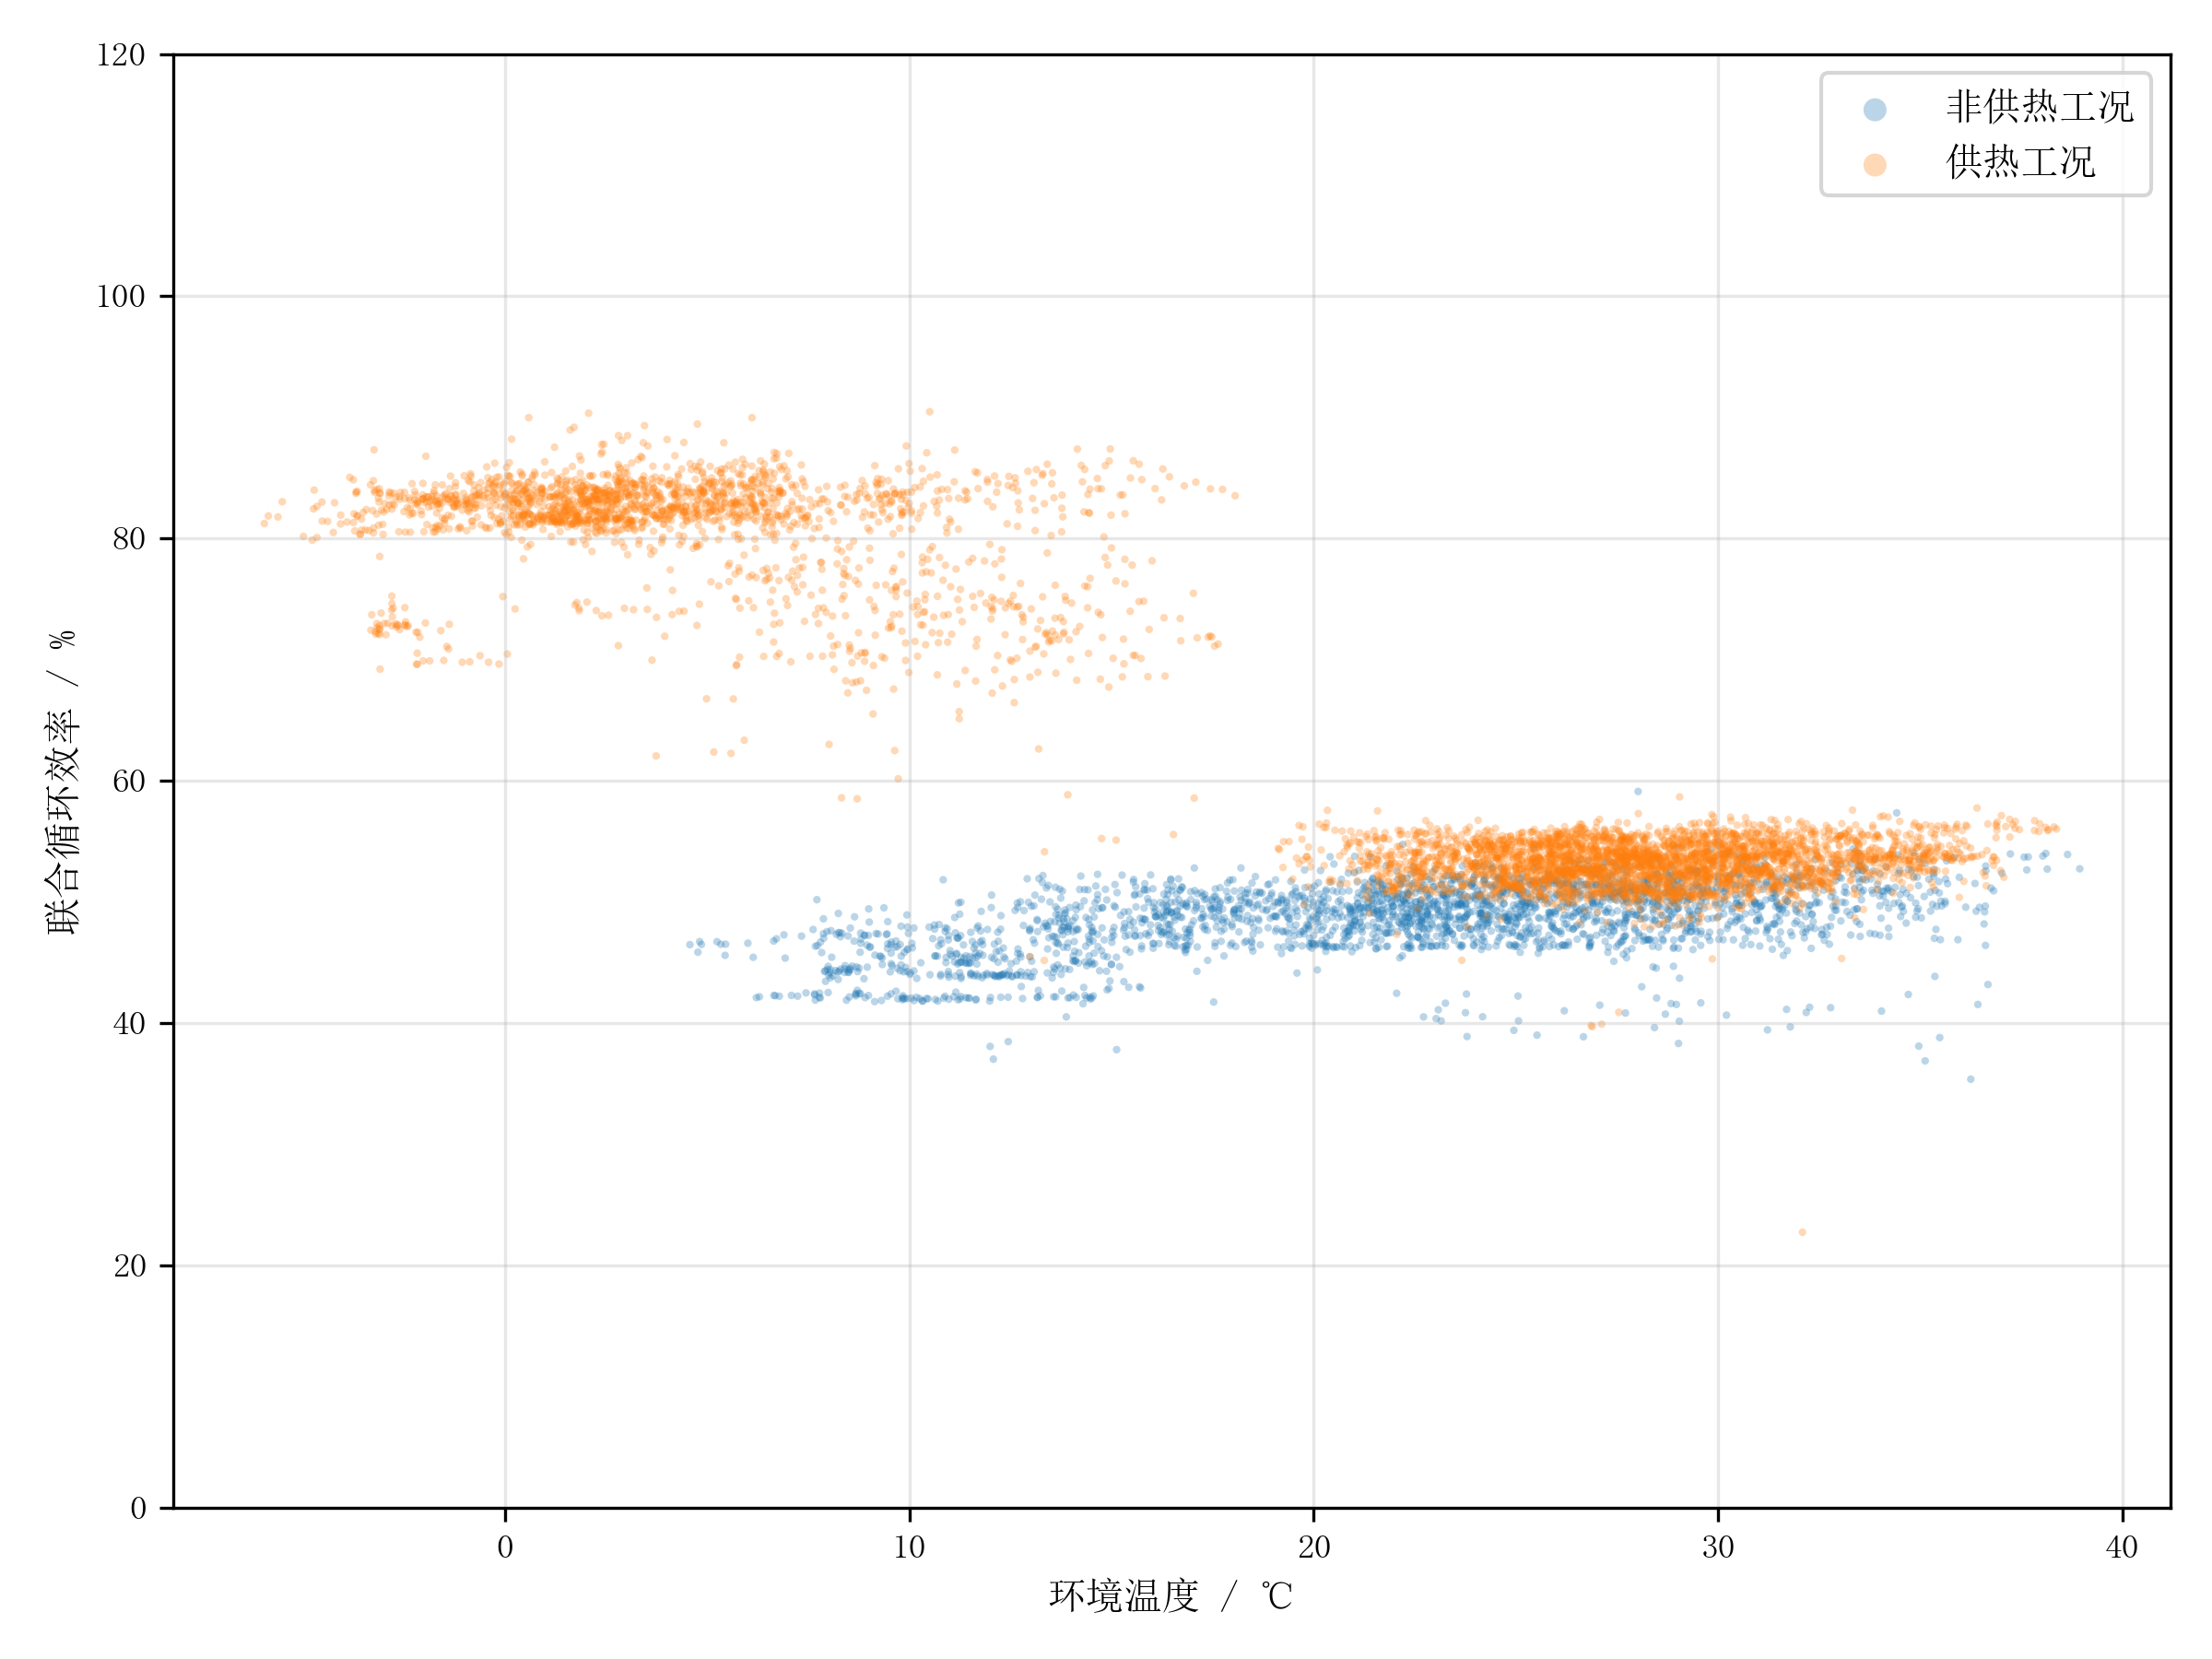
\includegraphics[width=\linewidth]{../../thesis/figures0/chapter5/环境温度_效率关系.png}
    \figcap{Fig. 8. Ambient temperature vs. efficiency.}
  \end{minipage}\hfill
  \begin{minipage}[t]{0.48\linewidth}
    \centering
    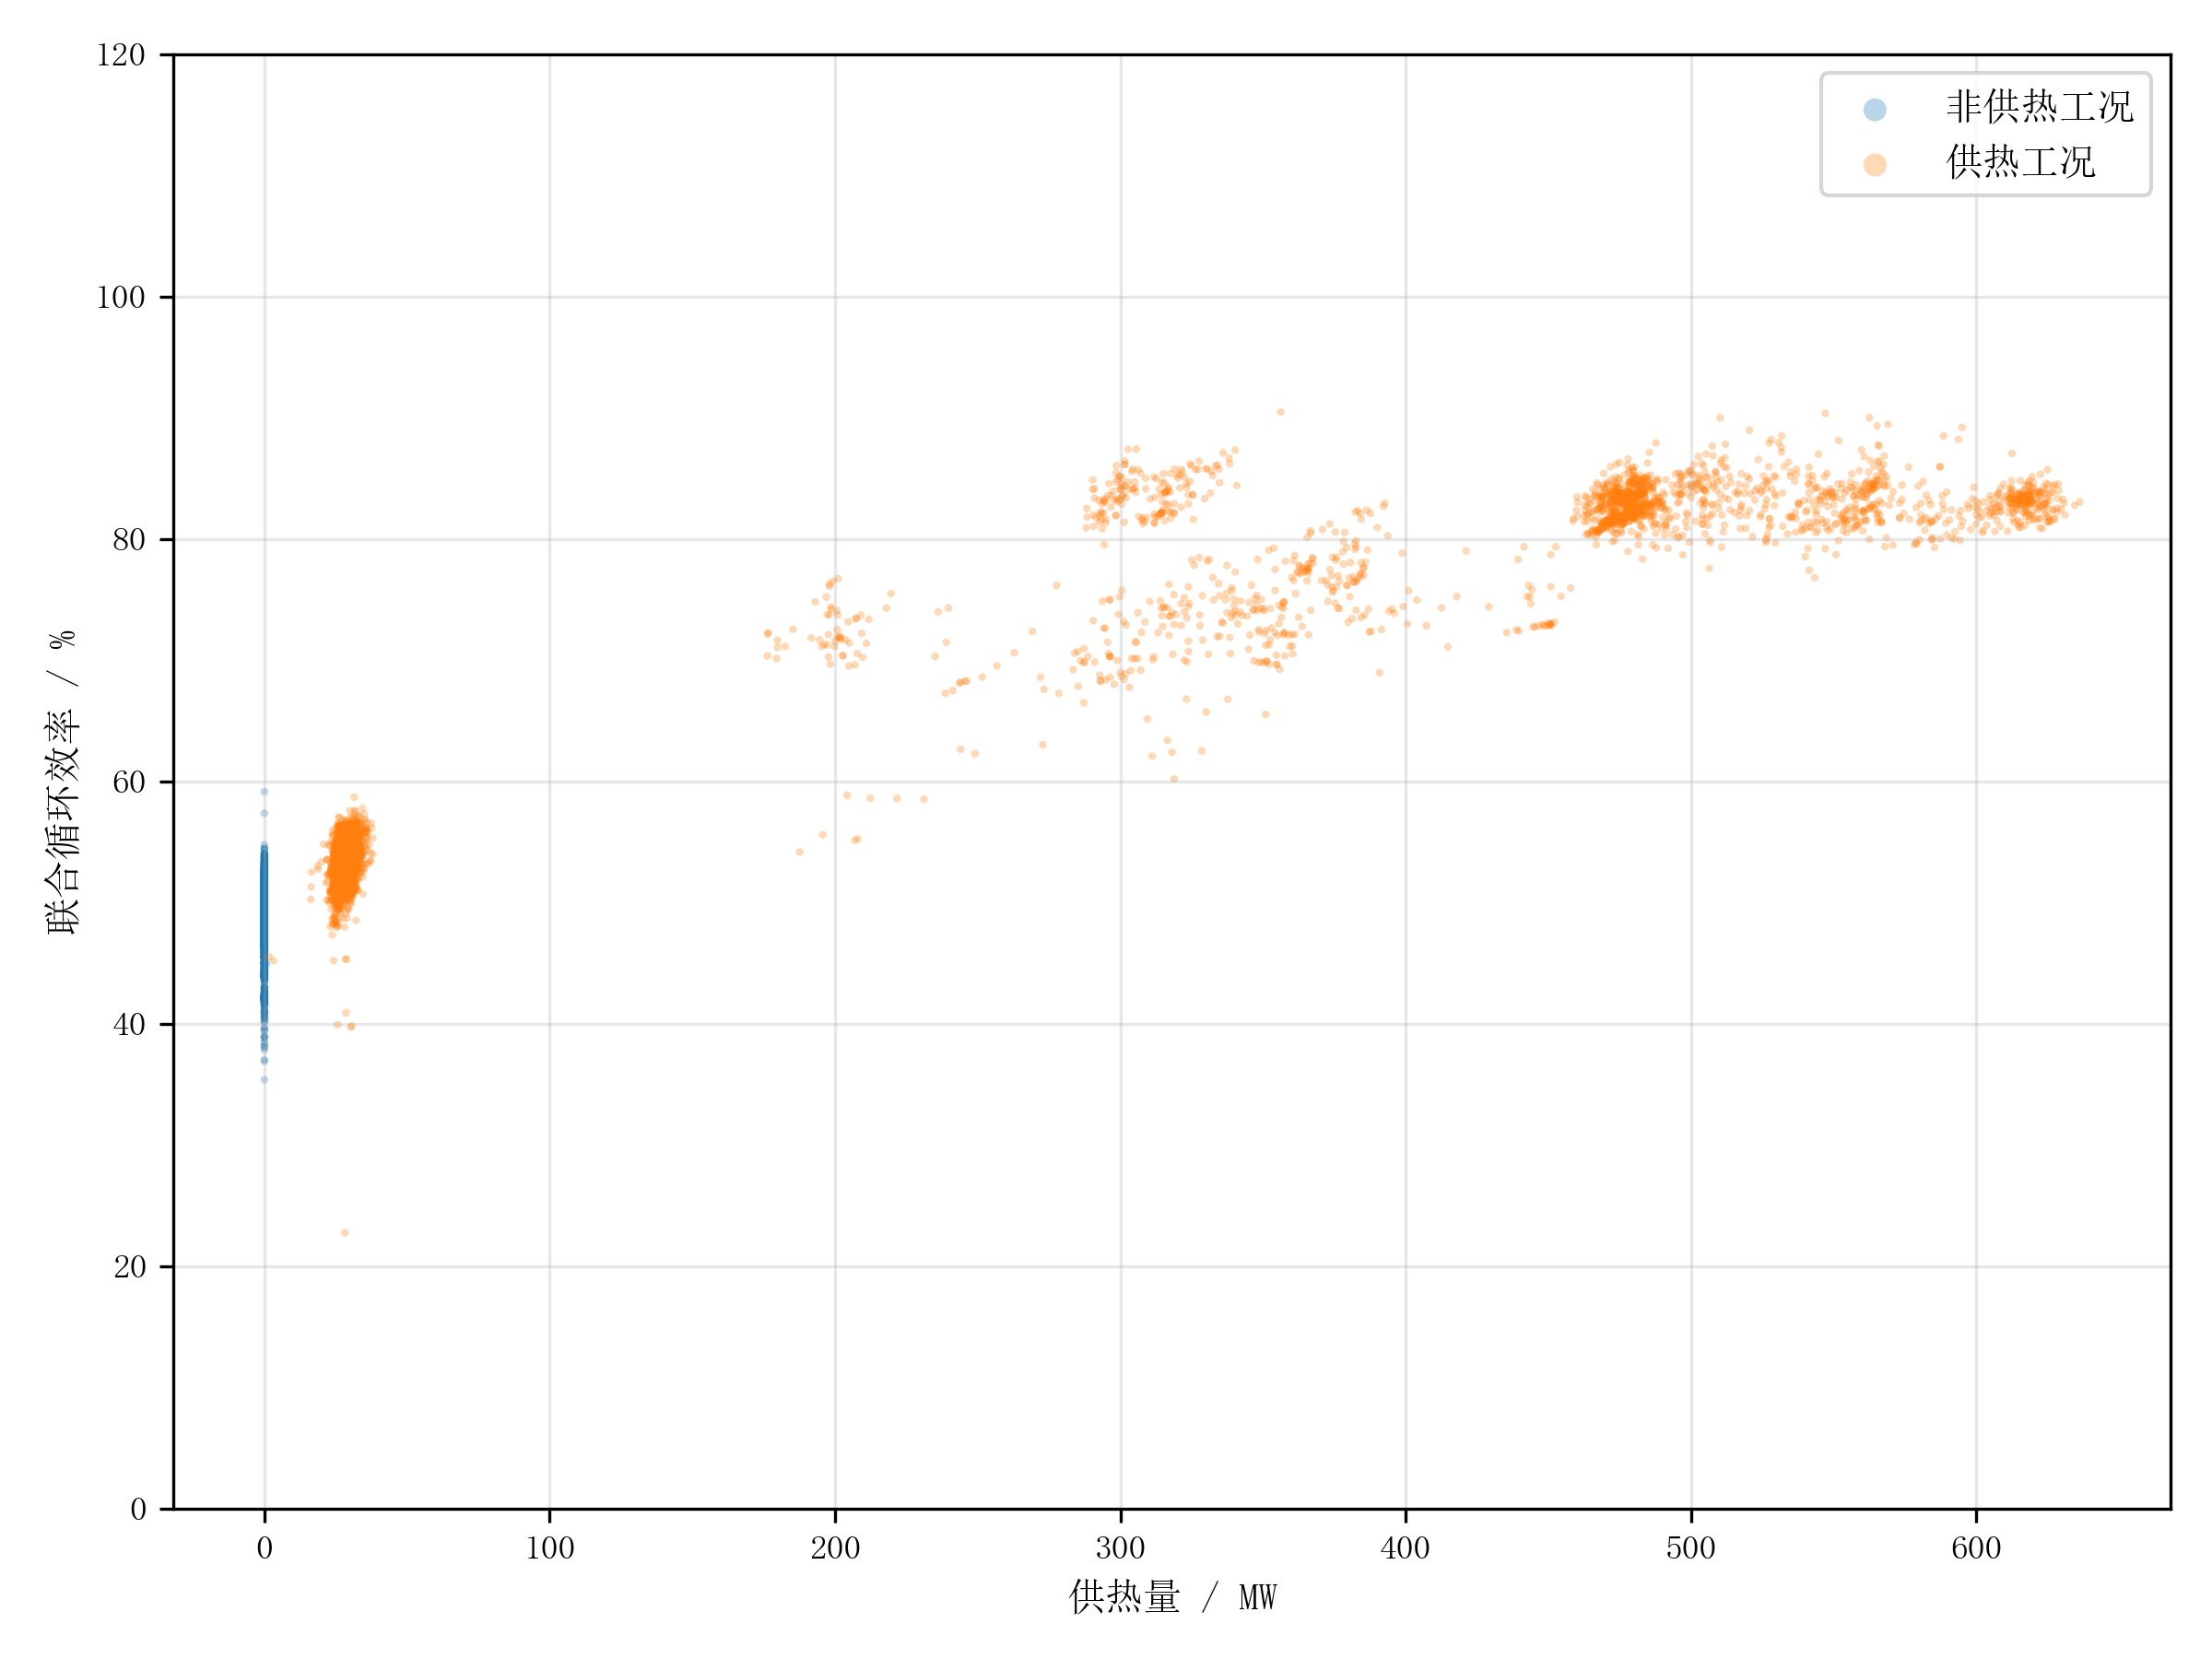
\includegraphics[width=\linewidth]{../../thesis/figures0/chapter5/供热量_效率关系.png}
    \figcap{Fig. 9. Heat supply vs. efficiency.}
  \end{minipage}

  \vspace{0.2em}
  \begin{minipage}[t]{0.48\linewidth}
    \centering
    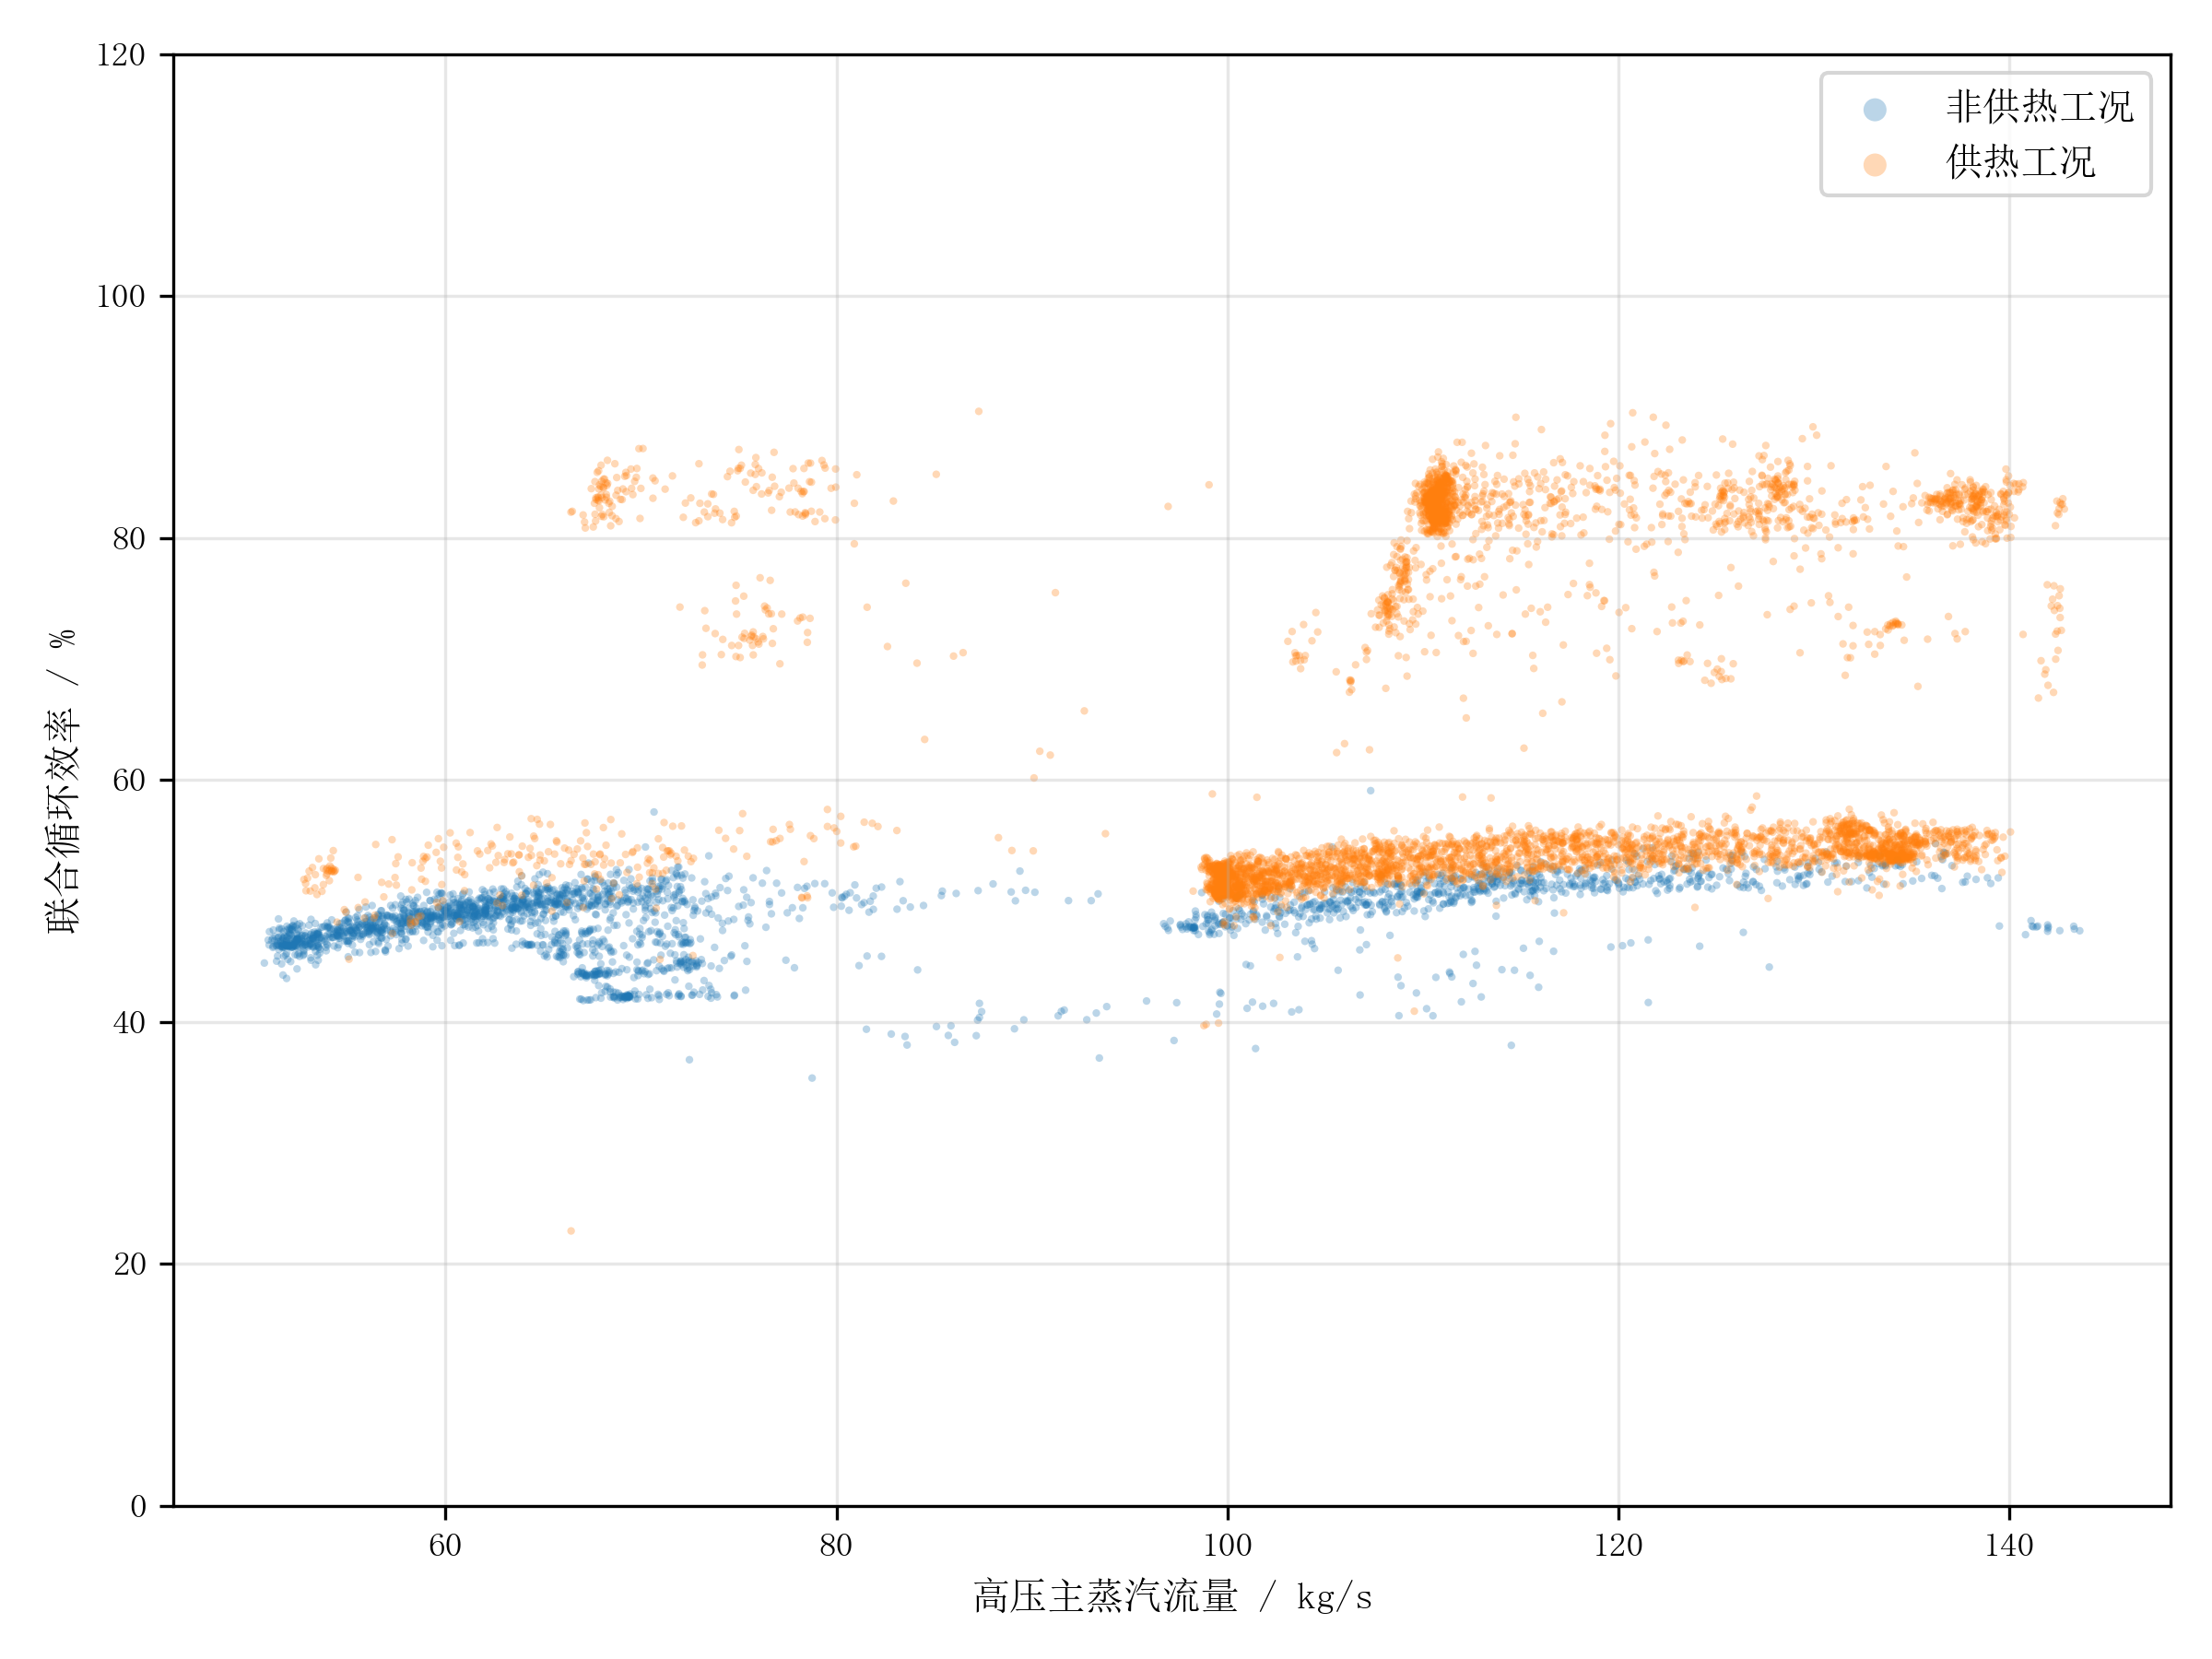
\includegraphics[width=\linewidth]{../../thesis/figures0/chapter5/高压主蒸汽流量_效率关系.png}
    \figcap{Fig. 10. HP main-steam flow vs. efficiency.}
  \end{minipage}\hfill
  \begin{minipage}[t]{0.48\linewidth}
    \centering
    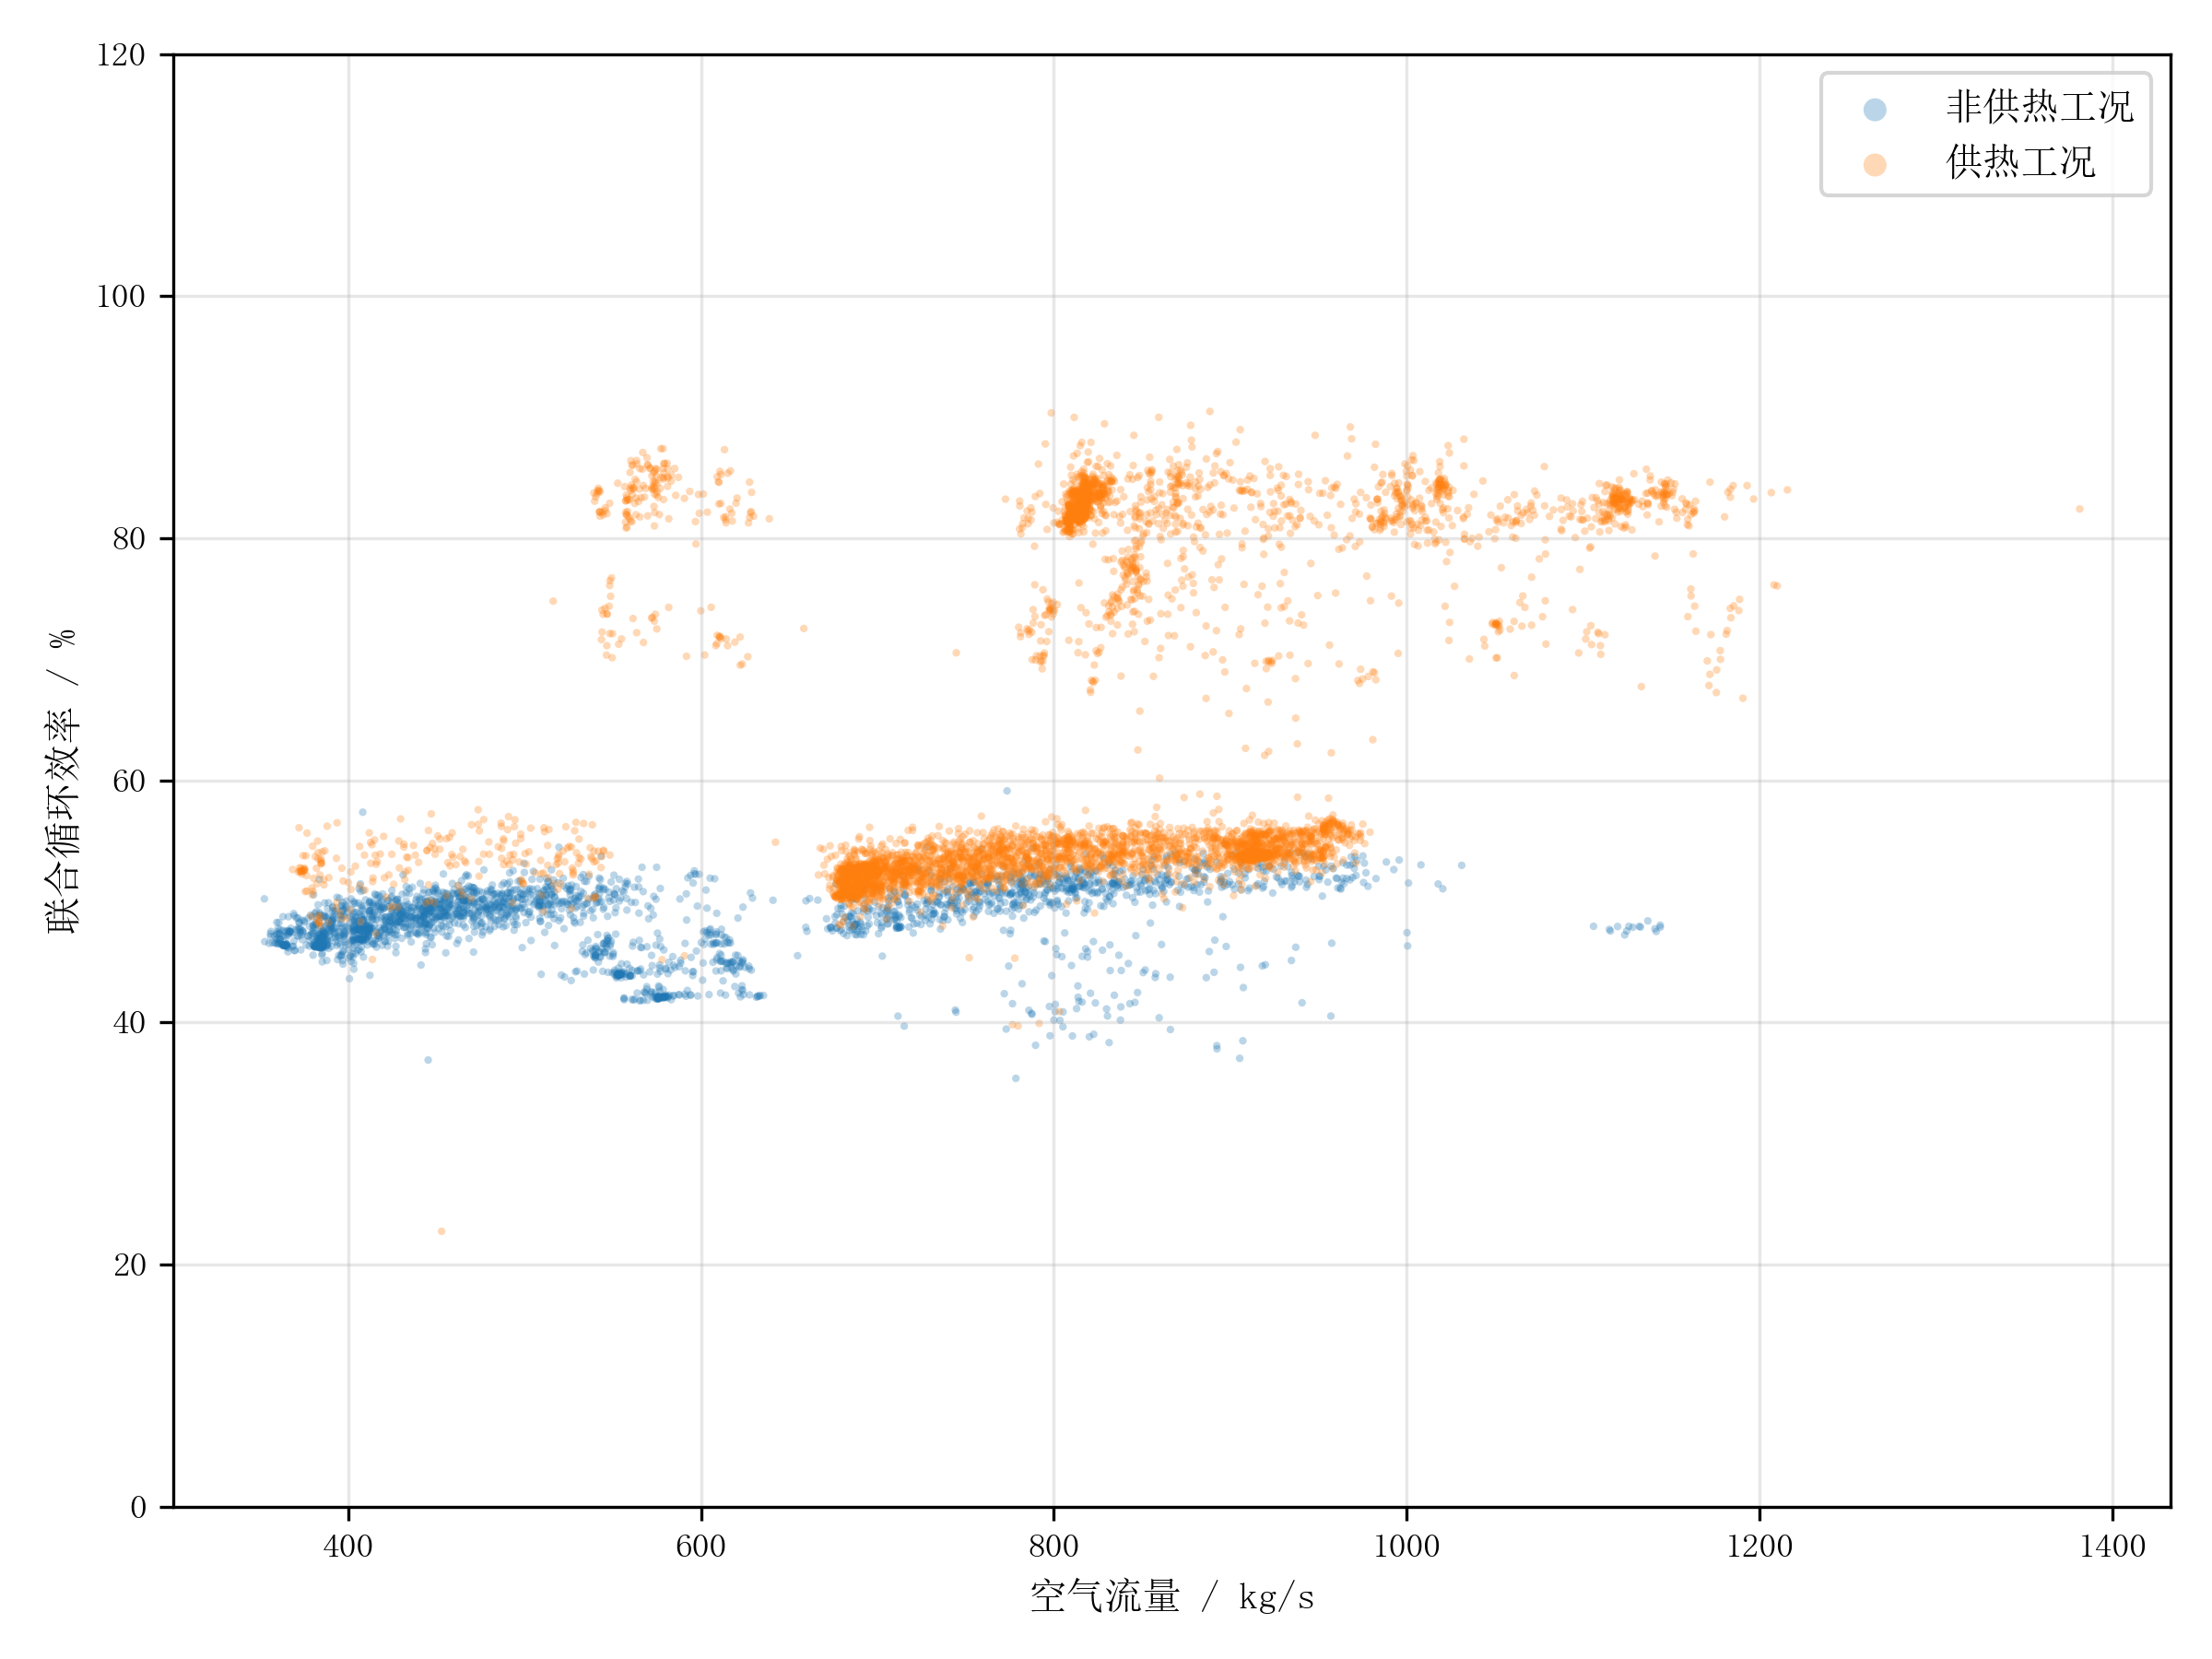
\includegraphics[width=\linewidth]{../../thesis/figures0/chapter5/空气流量_效率关系.png}
    \figcap{Fig. 11. Air flow vs. efficiency.}
  \end{minipage}
\end{center}
\end{sectionbox}

\vfill

\begin{sectionbox}{6. Summary and Future Work}
\smallbodyfont
\begin{itemize}
  \item A unified flow-state framework supports component-level and plant-level energy analysis from field data.
  \item GT analysis quantifies fuel-energy distribution among power output, compressor work, and exhaust heat.
  \item HRSG and ST analysis links water-side heat absorption with cylinder power and heating extraction.
\end{itemize}
\end{sectionbox}

\end{minipage}

\vfill
\color{theme}\rule{\linewidth}{0.8mm}

\end{document}
